\documentclass[a4paper, 12pt]{article}
% ABNT
\usepackage[top=2cm, bottom=2cm, left=2.5cm, right=2.5cm]{geometry}
\usepackage[onehalfspacing]{setspace} % Espaçamento de 1,5
\usepackage[T1]{fontenc}
\usepackage[brazil]{babel} % Traduzir para PT-BR
\usepackage{multirow}
% Pacotes essenciais
\usepackage[utf8]{inputenc} % Permite utilizar caracteres especiais: Ex: ç á à...
\usepackage{amsmath, amsfonts, amssymb}
\usepackage{float}
\usepackage{graphicx} % p/ add gráficos
\usepackage{IEEEtrantools} % Para fazer boas equações
\usepackage{float} % Poder usar a posição H no figure
% Introduzindo comandos utilizados
\usepackage{pgffor} % Pacote para laço condicional
\usepackage{textgreek}

% Comando para iniciar o cabeçao
\newcommand{\initcab}[2]{

\begin{tabular}{lllll}
	\multirow{4}*{\includegraphics[width=50px]{figs/logo_ufc.png}}    &			\multicolumn{4}{l}{\Large{\textbf{Universidade Federal do Ceará}}} \\
																	&			Disciplina:&\multicolumn{2}{l}{Processamento Estatístico de Sinais}\\
																	&			Professor:&Charles Casimiro Cavalcante \\
																	&			Estudante:&Rubem Vasceconcelos Pacelli & Matrícula: 474725 &
\end{tabular}

\begin{flushright}
\footnotesize{#1 de 2019}
\end{flushright}

{\Large Lista #2}

}

% Comando para a craiação de Rx
\newcommand{\RxTres}{
\begin{bmatrix}
 R_{dx}(0)  & R_{dx}(1)  & R_{dx}(2)\\
 R_{dx}(-1) & R_{dx}(0)  & R_{dx}(1)\\
 R_{dx}(-2) & R_{dx}(-1) & R_{dx}(0)\\
\end{bmatrix}
}

\newcommand{\RxTresE}{
\begin{bmatrix}
 \textEpsilon\left[ x^{2}\left[ n\right] \right] & 
 \textEpsilon\left[ x\left[ n\right] x\left[ n-1\right] \right] &
 \textEpsilon\left[ x\left[ n\right] x\left[ n-2\right] \right] \\
 \textEpsilon\left[ x\left[ n-1\right] x\left[ n\right] \right] &
 \textEpsilon\left[ x^{2}\left[ n-1\right] \right] &
 \textEpsilon\left[ x\left[ n-1\right] x\left[ n-2\right] \right] \\
 \textEpsilon\left[ x\left[ n-2\right] x\left[ n\right] \right] &
 \textEpsilon\left[ x\left[ n-2\right] x\left[ n-1\right] \right] &
 \textEpsilon\left[ x^{2}\left[ n-2\right] \right]
\end{bmatrix}
}


\newcommand{\RxDois}{
\begin{bmatrix}
 R_x(0)  & R_x(1)\\
 R_x(-1) & R_x(0)\\
\end{bmatrix}
}

\newcommand{\RxDoisE}{
\begin{bmatrix}
 \textEpsilon\left[ x^{2}\left[ n\right] \right] & 
 \textEpsilon\left[ x\left[ n\right] x\left[ n-1\right] \right] \\
 \textEpsilon\left[ x\left[ n-1\right] x\left[ n\right] \right] &
 \textEpsilon\left[ x^{2}\left[ n-1\right] \right]
\end{bmatrix}
}

\newcommand{\RdxDois}{
\begin{bmatrix}
 R_{dx}(0)\\
 R_{dx}(-1)\\
\end{bmatrix}
}

\newcommand{\RdxDoisE}{
\begin{bmatrix}
 \textEpsilon\left[ x\left[ n\right]d\left[ n\right] \right] &  \\
 \textEpsilon\left[ x\left[ n-1\right] d\left[ n\right] \right]
\end{bmatrix}
}
% Alguns comas
\newcommand{\R}{\tilde{R}}
\newcommand{\Rc}{\tilde{R}^{\,c}}
\newcommand{\np}{\textit{Neyman-Pearson}}
\newcommand{\hz}{H_0}
\newcommand{\hu}{H_1}
\newcommand{\lrf}{\textit{likelihood ratio function}}
\newcommand{\Q}{\mathnormal{Q}}
\newcommand{\y}{\mathbf{Y}}

\begin{document}

\initcab{Novembro}{5}

\begin{enumerate}

\item \label{q1}
	\begin{enumerate}
		\item
		Considere o seguinte teste de hipótese binária:
		\begin{IEEEeqnarray}{rCl}
			\IEEEyesnumber\label{h0h1}
			H_1: Y & = & S+N \IEEEyessubnumber  \label{h1}\\
			H_0: Y & = & N	 \IEEEyessubnumber  \label{h0}
		\end{IEEEeqnarray}
	Uma aplicação clássica da teoria de detecção é na área de radar. O enunciado dessa questão pode ser interpretado, para fins de contextualização, como um problema de detecção de um alvo em sistemas de sonar\slash radar. Sendo assim, consideraremos que $N$ é um ruído que corrompe a detecção de um alvo $S$.
	
	$H_0$ é denominada de \textit{null hypothesis} e indica a hipótese na qual não há a presença do alvo. $H_1$, por outro lado, é denominado de \textit{alternative hypotesis}, e indica a hipótese da sua presença.
	
	O estudo do teste de hipótese binários pode ser enunciado da seguinte forma: Dado um par de hipóteses ($\hu$ e $\hz$), deseja-se delimitar duas regiões ($\R$ e $\Rc$) no espaço amostral de $Y$, onde se aceita uma hipótese e se rejeita a outra. O particionamento das duas regiões é feito comparando um parâmetro $\theta$ da variável aleatória $Y$ com uma métrica, que é utilizado como regra de decisão. O método para se calcular a métrica, por sua vez, depende do tipo de teste de hipótese que é adotado (e.g., Neyman-Pearson, MAP, Bayes, MinMax). Além dissso, a forma que é separada as duas regiões (em \textit{one-tailed} ou \textit{two-tailed}) também modifica o valor final da métrica \cite{LeonGarcia}. Sendo assim, o estudo de detecção se resume em quatro passos importantes: \begin{enumerate}
	\item Definir o parâmetro $\theta$ a ser utilizado na detecção.
	\item Definir o teste de hipótese a ser adotado na questão.
	\item Definir como as regiões de decisão serão particionadas
	\item Calcular a métrica que será utilizada como métrica de decisão. \end{enumerate}
	
	% Falta dizer que eles são Simple alternatives: Dizer no passo 3
	% Falta dizer que theta é desconhecido mas não aleatório: Dizer no passo 2
	
	Primeiro: É necessário descobrir qual parâmetro de $Y$ muda entre as duas hipóteses para que possamos estima-la e, por fim, detectar a presença\slash ausência do alvo. Dado que $H_0$ seja verdadeiro, temos que sua média é:
	\begin{IEEEeqnarray}{rCl}
			E\left\lbrack y|H_0 \right\rbrack & \triangleq & \int_{-\infty }^{\infty } y\;f_Y \left(y\right)\;\mathrm{dy} \nonumber \\
			& = & \int_{-2 }^{2 } n\;f_N \left(n\right)\;\mathrm{dn}\nonumber \\
			& = & 0
		\end{IEEEeqnarray}
		
		E sua variância é:
		\begin{IEEEeqnarray}{rCl}
			\mathrm{VAR}\left\lbrack Y|H_0 \right\rbrack & \triangleq & \int_{-\infty }^{\infty } y^2 \;f_Y \left(y\right)\;\mathrm{dy} \nonumber \\
			& = & \int_{-2}^2 n^2 \;f_N \left(n\right)\;\mathrm{dn} \nonumber \\
			& = & \frac{4}{3}
		\end{IEEEeqnarray}
		
		Por outro lado, se $H_1$ for verdadeiro, então:
		\begin{IEEEeqnarray}{rCl}
			E\left\lbrack y|H_1 \right\rbrack & \triangleq &\int_{-\infty }^{\infty } y\;f_Y \left(y\right)\;\mathrm{dy} \nonumber \\
			& = & \int_{-1 }^{1 } s\;f_S \left(n\right)\;\mathrm{ds}+\int_{-2 }^{2 } n\;f_N \left(n\right)\;\mathrm{dn} \nonumber \\
			& = & 0
		\end{IEEEeqnarray}
		
		E
		\begin{IEEEeqnarray}{rCl}
			\mathrm{VAR}\left\lbrack Y|H_1 \right\rbrack & \triangleq & \int_{-\infty }^{\infty } y^2 \;f_Y \left(y\right)\;\mathrm{dy} \nonumber \\
			& = & \int_{-2}^2 s^2 \;f_S \left(s\right)\;\mathrm{ds}+\int_{-2}^2 n^2 \;f_N \left(n\right)\;\mathrm{dn} \nonumber \\
			& = & \frac{5}{3}
			\label{varH1}
		\end{IEEEeqnarray}
				
	A segunda igualdade da equação \ref{varH1} se deve ao fato de que $S$ e $N$ são viráveis aleatórias independentes, portanto $\mathrm{VAR}\left\lbrack S+N\right\rbrack =\mathrm{VAR}\left\lbrack S\right\rbrack +\mathrm{VAR}\left\lbrack N\right\rbrack$. Observe que, enquanto que a média permanece inalterada para as duas hipóteses, a variância de $Y$ muda. Portanto, defini-se o parâmetro para a detecção de presença\slash ausência de alvo como $\theta=\mathrm{VAR}\left\lbrack Y\right\rbrack=\sigma_Y^2$. Com isso, montamos o seguinte enunciado:
	\begin{IEEEeqnarray}{rCl}
			H_0 & : & Y\;\mathrm{e}\;\mathrm{uma}\;\mathrm{V}\ldotp \mathrm{A}\;\mathrm{com}\;\mu_Y  =0\;\mathrm{e}\;\sigma_Y^2 =\theta =4/3 \nonumber \\
			H_1 & : & Y\;\mathrm{e}\;\textrm{uma}\;\mathrm{V}\ldotp \mathrm{A}\;\textrm{com}\;\mu_Y =0\;\mathrm{e}\;\sigma_Y^2 =\theta =5/3
		\end{IEEEeqnarray}
	
	Segundo: É necessário adotarmos um teste de hipótese para calcularmos a métrica a ser utilizada como regra de decisão. É importante constatar que o parâmetro utilizado para a detecção é um valor desconhecido mas não aleatório. Métodos Bayseanos e o método a máxima posteriori (MAP) são utilizados em situações em que o parâmetro selecionado para a métrica é aleatório e, portanto, não é adequado para o presente problema \cite{LeonGarcia} \cite{SteveMKayDois}. O enunciado da questão solicita para que seja utilizado a função da razão do teste de verossimilhança (ou do inglês, \lrf). O teste de hipótese \np ~é o mais apropriado para essa questão, uma vez que ele utiliza a \lrf ~para obter a métrica.
	
	Terceiro: É necessário definirmos como se pretende dividir a região de rejeição ($\R$) e a região de aceitação ($\Rc$). É interessante observar que tanto $\hz$ quanto $\hu$ são \textit{simple hypothesis}, pois ambas especificam a distribuição de $Y$ completamente, i. e., o parâmetro $\theta$ não está definido em termos de desigualdade ou diferença \cite{LeonGarcia} \cite{MouradBarkat}. Nesse tipo de situação, adota-se o particionamento das regiões em \textit{one-tailed}.
	
	Quarto: O enunciado já fixou previamente três possíveis valores de limiar: $\eta=1/4$, $\eta=1$ e $\eta=2$. Pelo teste de hipótese de \np , dado um nível de significância (também chamado de probabilidade de falso alarme)
	\begin{IEEEeqnarray}{rCl}
			\alpha & = P\left\lbrack D_1 |H_0 \right\rbrack & =\int_{y|\Lambda \left(y\right)\ge \eta }^{\;} f_Y \left(y|H_0 \right)\mathrm{dy}
			\label{alpha}
	\end{IEEEeqnarray}
		
	Em que $\Lambda \left(y\right)$ é \lrf
	\begin{IEEEeqnarray}{rCl}
			\Lambda \left(y\right) & = & \frac{f_Y \left(y|H_1 \right)}{f_Y \left(y|H_0 \right)}
			\label{lrf}
	\end{IEEEeqnarray}
	
	Escolhe-se um valor de $\eta$ que minimize o valor de a probabilidade de \textit{miss}
	\begin{IEEEeqnarray}{rCl}
			\beta & = & P\left\lbrack D_0 \left|H_1 \right.\right\rbrack
			\label{beta}
	\end{IEEEeqnarray}
	
	Observe que
	\begin{IEEEeqnarray}{rClCr}
			f_Y \left(y|H_0 \right) & = & f_N \left(n\right) & = \frac{1}{4} &\qquad\quad\mathnormal{para}\;\,\vert y\vert \geq 2
			\label{fyH0}
	\end{IEEEeqnarray}
	
	E que 
	\begin{IEEEeqnarray}{rCl}
			f_Y \left(y|H_1 \right) & = & f_Y \left(y\left|H_1 \right.\right)=f_N \left(n\right)\ast f_S \left(s\right)
			\label{fyH1}
	\end{IEEEeqnarray}
	
	Em que $\ast$ indica a operação de convolução. A equação \ref{fyH1} segue do fato de que a função densidade de probabilidade (PDF) da soma de duas variáveis aleatórias independentes é igual a integral de convolução da PDF das mesmas \cite{LeonGarcia}. Resolvendo a integral de convolução em \ref{fyH1}, têm-se que:
	\begin{IEEEeqnarray}{rCl}
			f_Y \left(y\left|H_1 \right.\right) & = & \left\lbrace \begin{array}{cl}
																	0 & \mathrm{para}\;|y|>3\\
																	\frac{y+3}{8} & \mathrm{para}\;-3<y<-1 \\
																	\frac{1}{4} & \mathrm{para}\;|y|\leq 1 \\
																	\frac{-y+3}{8} & \textrm{para}\;1<y<3
																  \end{array}\right.
			\label{fyH1r}
	\end{IEEEeqnarray}
	
	Substituindo as equações \ref{fyH1r} e \ref{fyH0} em \ref{lrf}, têm-se
	\begin{IEEEeqnarray}{rCl}
			\Lambda \left(y\right)  & = & \left\lbrace \begin{array}{cl}
																	\frac{y+3}{2} & \mathrm{para}\;-2<y<-1 \\
																	1 & \mathrm{para}\;|y|\leq 1 \\
																	\frac{-y+3}{2} & \textrm{para}\;1<y<2
																  \end{array}\right.
			\label{lrfr}
	\end{IEEEeqnarray}
	
	$\Lambda \left(y\right)$ não é definido fora desse intervalo. O critério de decisão do teste de hipótese é \np~é dado por:
	\begin{IEEEeqnarray}{rCl}
			\Lambda \left(y\right)  & \begin{array}{cl}
											\hu \\
											>\\
											< \\
											\hz \end{array}    & \eta
			\label{cdd}
	\end{IEEEeqnarray}
	
	A região em que se aceita $\hz$ é denotada por $\Rc$, enquanto que a região em que se aceita $\hu$ é denotada por $\R$ . Sendo assim, define-se as regiões como
		\begin{IEEEeqnarray}{lCl}
			\IEEEyesnumber \label{rRcBoth}
			\R & = &  {y\; |\;\Lambda \left(y\right)>\eta} \IEEEyessubnumber \label{R} \\
			\Rc & = & {y\; |\;\Lambda \left(y\right)<\eta} \IEEEyessubnumber \label{Rc}
		\end{IEEEeqnarray}
	Para cara um dos valores dados para $\eta$ , basta substituí-los em \ref{cdd}. 
	\item
		O enunciado do teste de hipótese de \np ~espera que o problema forneça $\alpha$ e, com isso, calcula-se $\eta$. No entanto, ao invés fornecer o valor de $\alpha$, o enunciado deu os valores de $\eta$. Portanto, faremos o caminho oposto calculando $\alpha$ para cada $\eta$. Da equação \ref{alpha} Temos que, para $\eta=1/4$
	\begin{IEEEeqnarray}{rCl}
			\alpha & = & \int_{y|\Lambda \left(y\right)\ge 1/4 }^{\;} f_Y \left(y|H_0 \right)\mathrm{dy} \nonumber \\
			& = & 1/4 \int_{-2}^{2} {dy} \nonumber \\
			& = & 1
			\label{n025}
	\end{IEEEeqnarray}
	
	O valores de $\eta$ escolhidos nessa questão fogem do intervalo de limiar esperado pela \lrf . Com $\eta=1/4$, todos os valores levarão à hipótese $\hu$ (ver equação \ref{lrfr} e \ref{cdd}). Para $\eta=1\;\mathrm{ou}\;2$, temos:
	\begin{IEEEeqnarray}{rCl}
		\alpha & = & \int_{y|\Lambda \left(y\right)\ge \eta }^{\;} f_Y \left(y|H_0 \right)\mathrm{dy} \nonumber \\
		& = & 0
		\label{n12}
	\end{IEEEeqnarray}
	
	Esse resultado já é esperado, uma vez que valores superiores a 1 estão fora do conjunto imagem da \lrf . Neste caso, todos os valores de $Y$ definidos no domínio dessa função serão menores do que 1 e 2. Logo, o decisor sempre irá optar por $\hz$. Como $\alpha \triangleq P\left\lbrack D_1 |H_0 \right\rbrack$, é coerente que $\alpha = 0$ pois nunca optaríamos por $D_1$.
	
	\end{enumerate}
	
	\item
	Considere o seguinte enunciado:
	\begin{IEEEeqnarray}{rCl}
			H_0 & : & Y\;\mathrm{e}\;\mathrm{uma}\;\mathrm{V}\ldotp \mathrm{A}\;\mathrm{Gaussiana}\;\mathrm{com}\;m_0  =0\;\mathrm{e}\;\sigma_Y^2 =1 \nonumber \\
			H_1 & : & Y\;\mathrm{e}\;\textrm{uma}\;\mathrm{V}\ldotp \mathrm{A}\;\mathrm{Gaussiana}\;\textrm{com}\;m_1 =1\;\mathrm{e}\;\sigma_Y^2 =1
	\end{IEEEeqnarray}
	
	Observe que o valor da média muda nas duas hipóteses. Portanto, $\theta=m_j$, para $j=0,1$. A função densidade de probabilidade variável aleatória Gaussiana é dado por
	\begin{IEEEeqnarray}{rCl}
		f_Y \left(y\right)=\frac{1}{\sqrt{2\pi }}e^{-\frac{{\left(y-m_j \right)}^2 }{2}}
	\end{IEEEeqnarray}
	
	Da equação \ref{lrf}, temos que a \lrf ~é:
	\begin{IEEEeqnarray}{rCl}
			\Lambda \left(y\right) & = & \frac{f_Y \left(y|H_1 \right)}{f_Y \left(y|H_0 \right)} \nonumber \\
			& = & \mathrm{exp}\left(\frac{{\left(y-m_0 \right)}^2 }{2}-\frac{{\left(y-m_1 \right)}^2 }{2}\right) \nonumber \\
			& = & \mathrm{exp}\left(\frac{{2y-1} }{2}\right)
			\label{lrfq2}
	\end{IEEEeqnarray}
	
	Aplicando o logaritmo natural nos dois lados da equação \ref{cdd}, temos:
		\begin{IEEEeqnarray}{rCl}
			\ln \Lambda \left(y\right)  & \begin{array}{cl}
											\hu \\
											>\\
											< \\
											\hz \end{array}    & \ln \eta \nonumber \\
			\frac{{2y-1} }{2}		   & \begin{array}{cl}
											\hu \\
											>\\
											< \\
											\hz \end{array}    & \ln \eta \nonumber \\
			y						   & \begin{array}{cl}
											\hu \\
											>\\
											< \\
											\hz \end{array}    & \frac{2\ln \eta+1}{2} = \gamma
			\label{cddq2}
	\end{IEEEeqnarray}
	
	O nível de significância é
	\begin{IEEEeqnarray}{rCl}
			\alpha & = & \int_{y|\ln\Lambda \left(y\right)\ge \ln\eta }^{\;} f_Y \left(y|H_0 \right)\mathrm{dy} \nonumber \\
			& = & \frac{1}{\sqrt{2\pi }} \int_{\gamma}^{\infty} e^{-\frac{y^2 }{2}} {dy} \nonumber \\
			& = & \Q\left(\gamma \right)
			\label{alphaq2}
	\end{IEEEeqnarray}
	
	Para $\alpha=0,005$, $\gamma=1,645$. Sendo assim, para realizar a decisão da variável aleatória $Y$ baseado na hipótese de teste de \np , basta comparar seu valor com 1,645 . Se for maior, deve-se decidir por $\hu$, caso contrário, decidi-se por $\hz$.
	
	\item
		Nessa questão, estamos interessados em saber a existência de um vetor de variáveis aleatórias $\y=\left[Y_1 Y_2 \cdots Y_K\right]$, para $1\leq k\leq K$ em que
	\begin{IEEEeqnarray}{rCl}
			H_0 & : & Y_k\;\mathrm{e}\;\mathrm{uma}\;\mathrm{V}\ldotp \mathrm{A}\;\mathrm{Gaussiana}\;\mathrm{com}\;m_0  =0\;\mathrm{e}\;\sigma_Y^2\;\mathrm{conhecido} \nonumber \\
			H_1 & : & Y_k\;\mathrm{e}\;\textrm{uma}\;\mathrm{V}\ldotp \mathrm{A}\;\mathrm{Gaussiana}\;\textrm{com}\;m_1 = m\;\mathrm{e}\;\sigma_Y^2\;\mathrm{conhecido}
	\end{IEEEeqnarray}
	
	Para $\hz$ verdadeiro, temos:
	\begin{IEEEeqnarray}{rCl}
			f_{\mathit{\mathbf{Y}}} \left(\mathit{\mathbf{y}}|H_0 \right) & = & \prod_{i=1}^K f_{Y_i } \left(y_i |H_0 \right) \nonumber \\
			& = & \frac{1}{{\left(\sigma \sqrt{2\pi }\right)}^K }\mathrm{exp}\left(-\frac{1}{2\sigma^2 }\sum_{i=1}^K {y_i }^2 \right)
	\end{IEEEeqnarray}
	
	Por outro lado, se $\hu$ for verdadeiro:
	\begin{IEEEeqnarray}{rCl}
			f_{\mathit{\mathbf{Y}}} \left(\mathit{\mathbf{y}}|H_1 \right) & = & \prod_{i=1}^K f_{Y_i } \left(y_i |H_1 \right) \nonumber \\
			& = & \frac{1}{{\left(\sigma \sqrt{2\pi }\right)}^K }\exp \left(-\frac{1}{2\sigma^2 }\sum_{i=1}^K {\left(y_i -m\right)}^2 \right)
	\end{IEEEeqnarray}
	
	A \lrf ~é dado por:
		\begin{IEEEeqnarray}{rCl}
			\Lambda \left(\mathbf{y}\right) & = & \frac{f_\mathbf{Y} \left(\mathbf{y}|H_1 \right)}{f_\mathbf{Y} \left(\mathbf{y}|H_0 \right)} \nonumber \\
			& = & \exp \left(-\frac{1}{2\sigma^2 }\sum_{i=1}^K \left(y_i -m\right)-{y_i }^2 \right) \nonumber \\
			& = & \exp \left(-\frac{1}{2\sigma^2 }\sum_{i=1}^K m^2 -2\mathit{my}\right)  \nonumber \\
			& = & \exp \left(-\frac{1}{2\sigma^2 }\left(Km^2 -2m\sum_{i=1}^K y\right)\right) \nonumber \\
			& = & \exp \left(-\frac{1}{2\sigma^2 }\left(Km^2 -2\mathrm{mK}\overline{Y_K } \right)\right)
			\label{lrfq3}
	\end{IEEEeqnarray}
	
	Em que $\overline{Y_K }$ é o estimador da média, dado por
	\begin{IEEEeqnarray}{rCl}
			\overline{Y_K } & = & \frac{1}{K}\sum_{i=1}^K \textrm{y}
			\label{yk}
	\end{IEEEeqnarray}
	
	Aplicando o logaritmo natural nos dois lados da equação \ref{cdd}, temos:
	\begin{IEEEeqnarray}{rCl}
			\ln \Lambda \left(y\right)  & \begin{array}{cl}
											\hu \\
											>\\
											< \\
											\hz \end{array}    & \ln \eta \nonumber \\
			-\frac{1}{2\sigma^2 }\left(Km^2 -2\mathrm{mK}\overline{Y_K }\right)		   & \begin{array}{cl}
																								\hu \\
																								>\\
																								< \\
																								\hz \end{array}    & \ln \eta \nonumber \\
			\overline{Y_K } 										 						   & \begin{array}{cl}
																								\hu \\
																								>\\
																								< \\
																								\hz \end{array}    & \frac{\sigma^2 \ln\eta }{\mathit{Km}}+\frac{m}{2}
																								\label{cddq3}
	\end{IEEEeqnarray}
	
	A equação \ref{cddq3} mostra que o critério de decisão baseado no teste de hipótese binário de \np ~utiliza a média estatística do vetor de variáveis aleatórias como métrica. Este resultado é plenamente coerente, uma vez que estamos utilizando a média dessa variável como parâmetro para a detecção.

\item
	Em todas as questões anteriores, estávamos realizando um teste de hipótese binário de um parâmetro $\theta$ desconhecido mas constante. A definição dos valores de $\theta$ feitas em $\hz$ e $\hu$ dizem respeito à suposições na qual essa constante poderia ser. Se o problema consistia em decidir se $\theta$ é igual a um de dois valores possíveis, era definido um par de \textit{simple hypothesis}. Caso fosse de interesse saber se a constante $\theta$ é diferente de um valor ou de um conjunto de valores, era definido uma \textit{composite hypothesis} em termos de diferença ou de inequação.

	Nesta questão, abordamos a teoria de detecção aplicada a telecomunicações com um novo enunciado do problema: Dado uma variável aleatória gaussiana $Y$, de média $\Theta$ e variância unitária, deseja-se determinar um limiar para a decisão do sinal recebido. No entanto, diferente das outras questões, $\Theta$ é uma variável aleatória discreta.
	
	Essa (não tão) sutil diferença implica diretamente no tipo de teste de hipótese que devemos usar. Como dito na \ref{q1}, o métodos Bayseanos e de MAP são utilizados quando o parâmetro a ser detectado é aleatório. O critério de Bayes utiliza o conceito de custo para a determinação do limiar de decisão enquanto o de MAP não. No entanto, os dois necessitam do conhecimento a priori ($p_\Theta(\theta)$). Como não foi fornecido o custo para esse problema, utilizaremos o teste de hipótese MAP.
	
	Seja a \lrf ~dada pela a equação \ref{lrf}, o teste de hipótese MAP fornece que:
	\begin{IEEEeqnarray}{rCl}
			\Lambda \left(y\right)  & \begin{array}{cl}
											\hu \\
											>\\
											< \\
											\hz \end{array}    & \frac{p_0}{p_1}
		\label{map}
	\end{IEEEeqnarray}
	
	Em que $p_0 = p_\Theta(-1)$ e $p_1 = p_\Theta(1)$. Portanto, seja a PDF do sinal recebido dado por:
	\begin{IEEEeqnarray}{rCl}
			f_Y \left(y\right)=\frac{1}{\sqrt{2\pi }}\exp \left(-\frac{1}{2}\sum_{i=1}^K {\left(y_i -\Theta \right)}^2 \right)
	\end{IEEEeqnarray}
	
	Podemos construir a seguinte par de hipóteses:
	\begin{IEEEeqnarray}{rCl}
			H_0 & : & Y\;\mathrm{e}\;\mathrm{uma}\;\mathrm{V}\ldotp \mathrm{A}\;\mathrm{Gaussiana}\;\mathrm{com}\;\theta_0  =-1\;\mathrm{e}\;\sigma_Y^2=1 \nonumber \\
			H_1 & : & Y\;\mathrm{e}\;\textrm{uma}\;\mathrm{V}\ldotp \mathrm{A}\;\mathrm{Gaussiana}\;\textrm{com}\;\theta_1 = 1\;\mathrm{e}\;\sigma_Y^2=1
	\end{IEEEeqnarray}
	
	Note que apenas o par de hipótese não fornece se $\Theta$ é uma variável aleatória, devemos conhecer o problema para saber se, de fato, é uma VA ou uma constante. O enunciado não fornece a probabilidade a priori do problema. Para contornar este problema, considera-se uma transmissão equiprovável ($p_0=p_1=0,5$). Se $\hz$ for verdadeira, temos:
	\begin{IEEEeqnarray}{rCl}
		f_Y \left(y|H_0 \right)=\frac{1}{\sqrt{2\pi }}\exp \left(-\frac{{\left(y_i +1\right)}^2 }{2}\right)
		\label{fyH0q4}
	\end{IEEEeqnarray}
	
	Por outro lado, se $\hu$ for verdadeira:
	\begin{IEEEeqnarray}{rCl}
		f_Y \left(y|H_0 \right)=\frac{1}{\sqrt{2\pi }}\exp \left(-\frac{{\left(y_i -1\right)}^2 }{2}\right)
		\label{fyH1q4}
	\end{IEEEeqnarray}
	
	Substituindo as equações \ref{fyH0q4} e \ref{fyH1q4} em \ref{map}, temos:
		\begin{IEEEeqnarray}{rCl}
			\exp \left(\frac{{\left(y_i +1\right)}^2 }{2}-\frac{{\left(y_i -1\right)}^2 }{2}\right)  & \begin{array}{cl}
											\hu \\
											>\\
											< \\
											\hz \end{array}    & 1 \nonumber \\
			\exp \left(2y\right)  & \begin{array}{cl}
											\hu \\
											>\\
											< \\
											\hz \end{array}    & 1
	\end{IEEEeqnarray}
	
	Aplicando o logaritmo natural nos dois lados da inequação, temos:
	\begin{IEEEeqnarray}{rCl}
			y  & \begin{array}{cl}
											\hu \\
											>\\
											< \\
											\hz \end{array}    & 0
			\label{cddq4}
	\end{IEEEeqnarray}
	
	O resultado chegado em \ref{cddq4} é intuitivo: Em uma comunicação binária, antipodal e equiprováveis, é intuitivo acreditar que o limiar de decisão seja 0. A Figura \ref{BERq4} mostra a taxa de erro de bits para diferentes valores de limiar $\eta$. Como é possível perceber, 0 é o valor de limiar que minimiza a taxa de erro de bits.
	\begin{figure}[H]
		\centering
		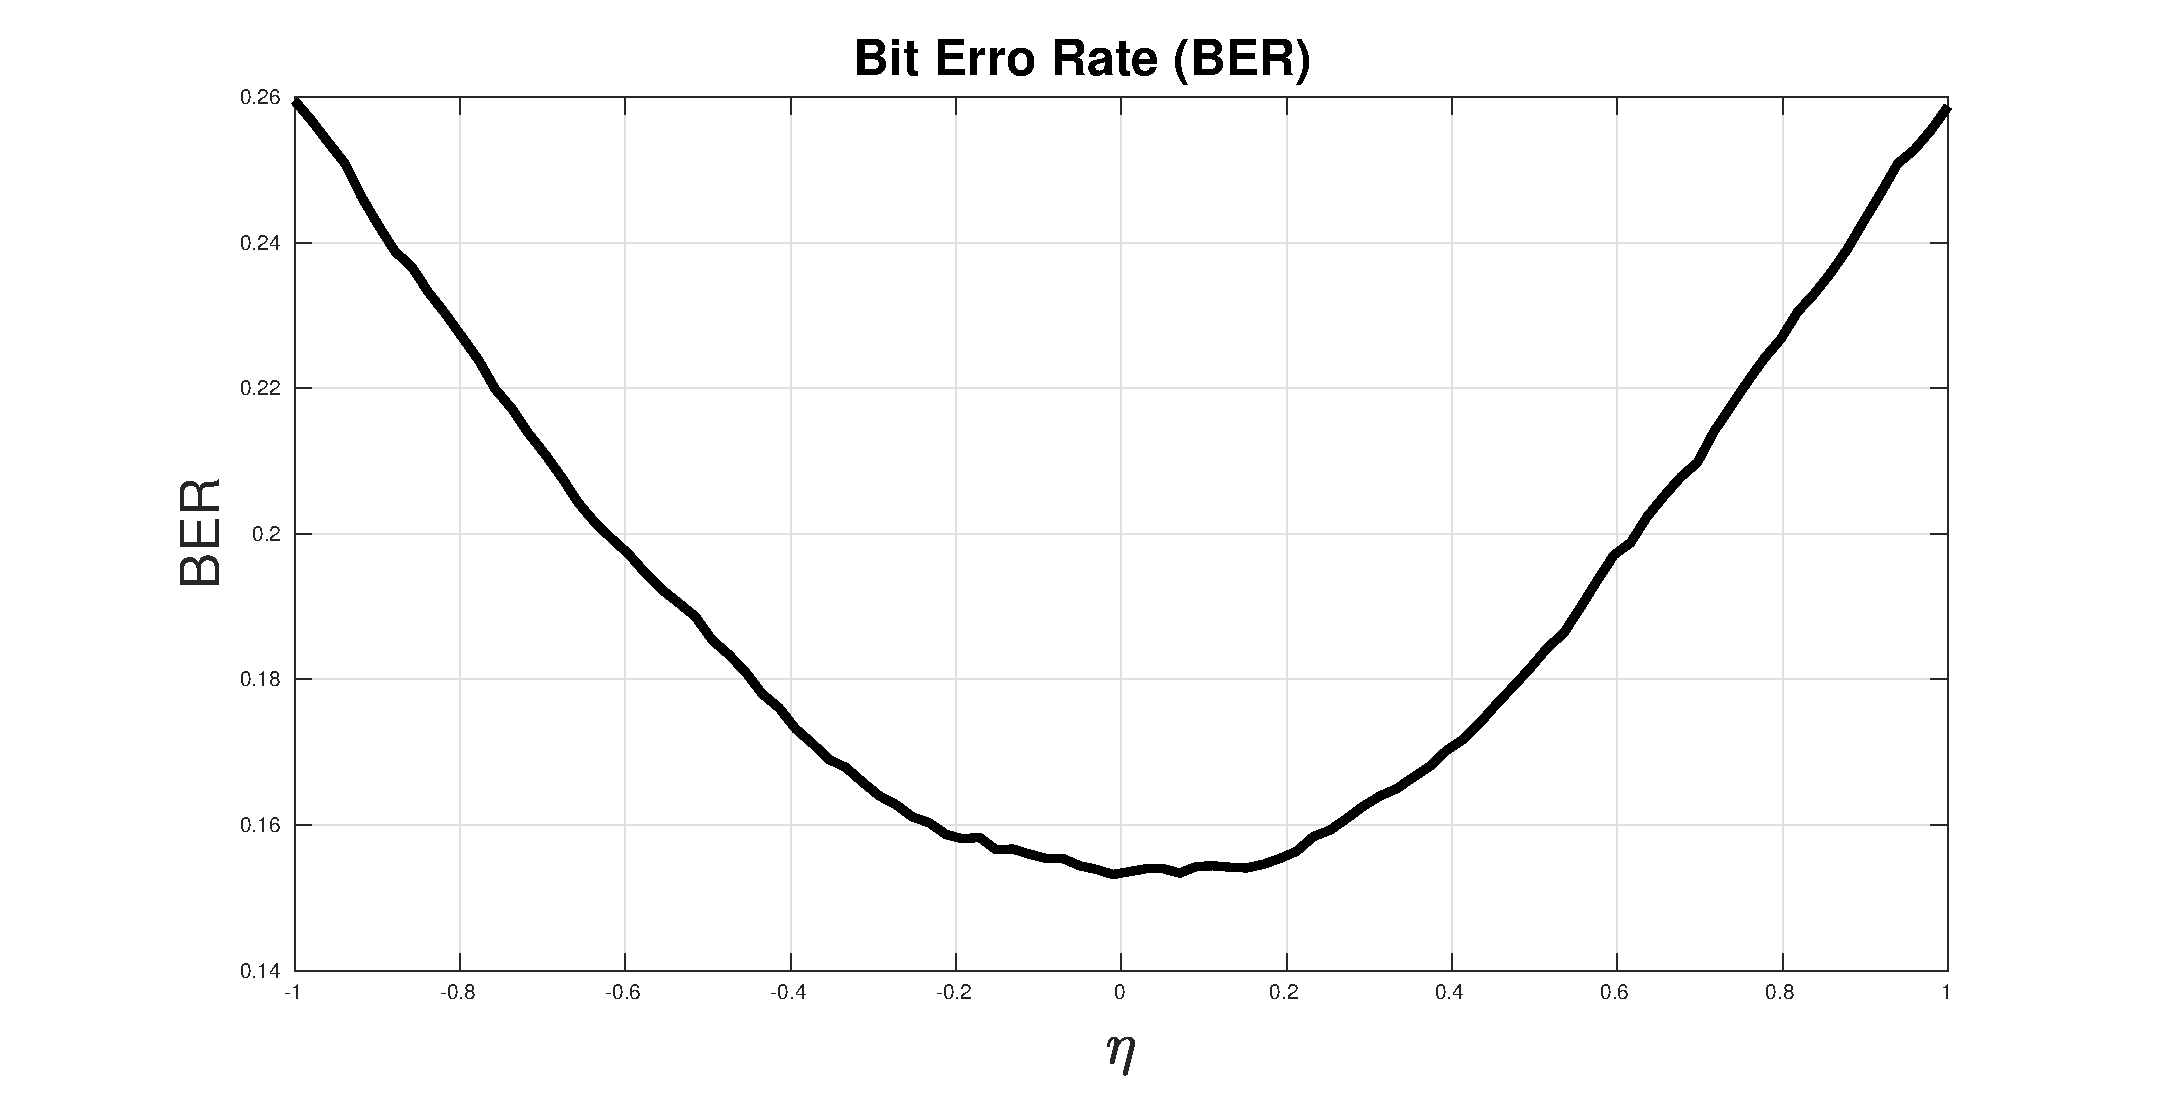
\includegraphics[scale=.4]{figs/BERq5.eps}
		\caption{Taxa de erro de bits para diferentes valores de limiar $\eta$.}
		\label{BERq4}
	\end{figure}
\end{enumerate}

\bibliography{ref.bib}
\bibliographystyle{ieeetr}

\end{document}